\section{Introduction}

Deep learning, as its name suggests, emerged from the idea of stacking more layers to achieve increased representation power and improved performance~\cite{Goodfellow-et-al-2016, He2015DeepRL}. However, despite the remarkable success of large language models, their core architecture is paradoxically shallow~\cite{strobl-2023}. This imposes a fundamental constraint on their most sought-after capability: reasoning. The fixed depth of standard Transformers places them in computational complexity classes such as $AC^0$ or $TC^0$~\cite{10.5555/1631171.1631212}, preventing them from solving problems that require polynomial time~\cite{MS-2023, Chiang-2025}. LLMs are not Turing-complete and thus they cannot, at least in a purely end-to-end manner, execute complex algorithmic reasoning that is necessary for deliberate planning or symbolic manipulation tasks~\cite{Lehnert2024BeyondAB, Bounsi2024TransformersMN}. For example, our results on the Sudoku task show that increasing Transformer model depth {\it can} improve performance,\footnote{Simply increasing the model width does not improve performance here.} but performance remains far from optimal even with very deep models (see \Cref{fig:perf-layers}), which supports the conjectured limitations of the LLM scaling paradigm~\citep{merrill-sabharwal-2023-parallelism}.

The LLMs literature has relied largely on Chain-of-Thought (CoT) prompting for reasoning~\cite{ChainOfThought2022}. CoT externalizes reasoning into token-level language by breaking down complex tasks into simpler intermediate steps, sequentially generating text using a shallow model~\cite{MS-2024}. However, CoT for reasoning is a crutch, not a satisfactory solution. It relies on brittle, human-defined decompositions where a single misstep or a misorder of the steps can derail the reasoning process entirely~\cite{Chen2024PremiseOM, Xu2024PreemptiveA}. This dependency on explicit linguistic steps tethers reasoning to 
patterns at the token level. As a result, CoT reasoning often requires significant amount of training data and generates a large number of tokens for complex reasoning tasks, resulting in slow response times. A more efficient approach is needed to minimize these data requirements~\cite{Villalobos2022WillWR}.

Towards this goal, we explore ``latent reasoning'', where the model conducts computations within its internal hidden state space~\cite{Chen2025ReasoningBL, CoconutLatentReasoning2024}. This aligns with the understanding that language is a tool for human communication, not the substrate of thought itself~\cite{fedorenko2024language}; the brain sustains lengthy, coherent chains of reasoning with remarkable efficiency in a latent space, without constant translation back to language. However, the power of latent reasoning is still fundamentally constrained by a model's \textit{effective computational depth}. Naively stacking layers is notoriously difficult due to vanishing gradients, which plague training stability and effectiveness~\citep{Goodfellow-et-al-2016, wang2024deepnet}. Recurrent architectures, a natural alternative for sequential tasks, often suffer from early convergence, rendering subsequent computational steps inert, and rely on the biologically implausible, computationally expensive and memory intensive Backpropagation Through Time (BPTT) for training~\cite{LILLICRAP201982}.

The human brain provides a compelling blueprint for achieving the effective computational depth that contemporary artificial models lack. It organizes computation hierarchically across cortical regions operating at different timescales, enabling deep, multi-stage reasoning~\citep{murray2014hierarchy, zeraati2023intrinsic, huntenburg2018large}. Recurrent feedback loops iteratively refine internal representations, allowing slow, higher-level areas to guide, and fast, lower-level circuits to execute—subordinate processing while preserving global coherence~\citep{lamme2000distinct, bastos2012canonical, kaleb2024feedback}. Notably, the brain achieves such depth without incurring the prohibitive credit-assignment costs that typically hamper recurrent networks from backpropagation through time~\citep{LILLICRAP201982, lillicrap2020backpropagation}.

\begin{figure}[t]
  \centering
  %  row
  \makebox[\linewidth][c]{%
    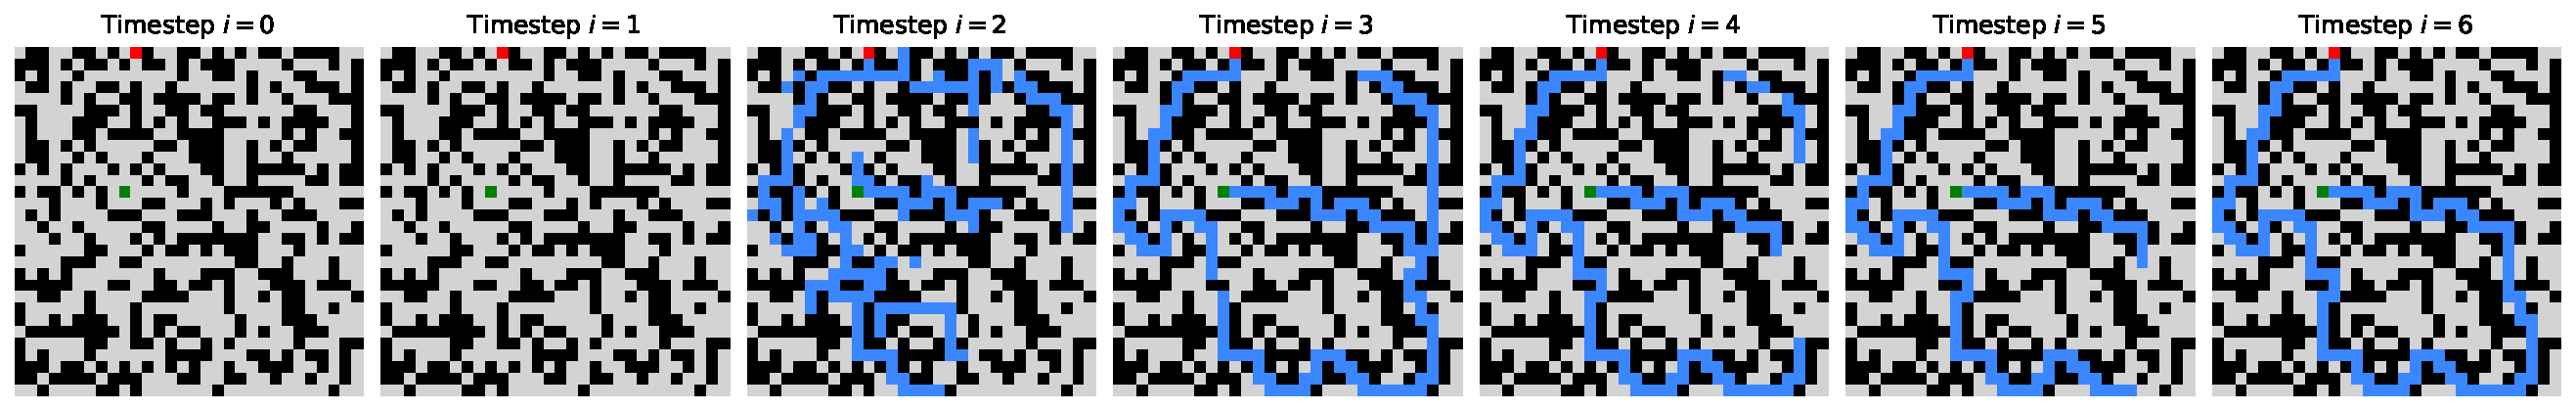
\includegraphics[width=1.1\linewidth]{figures/visualization/maze-100.pdf}%
  }\\
  % row
  \makebox[\linewidth][c]{%
    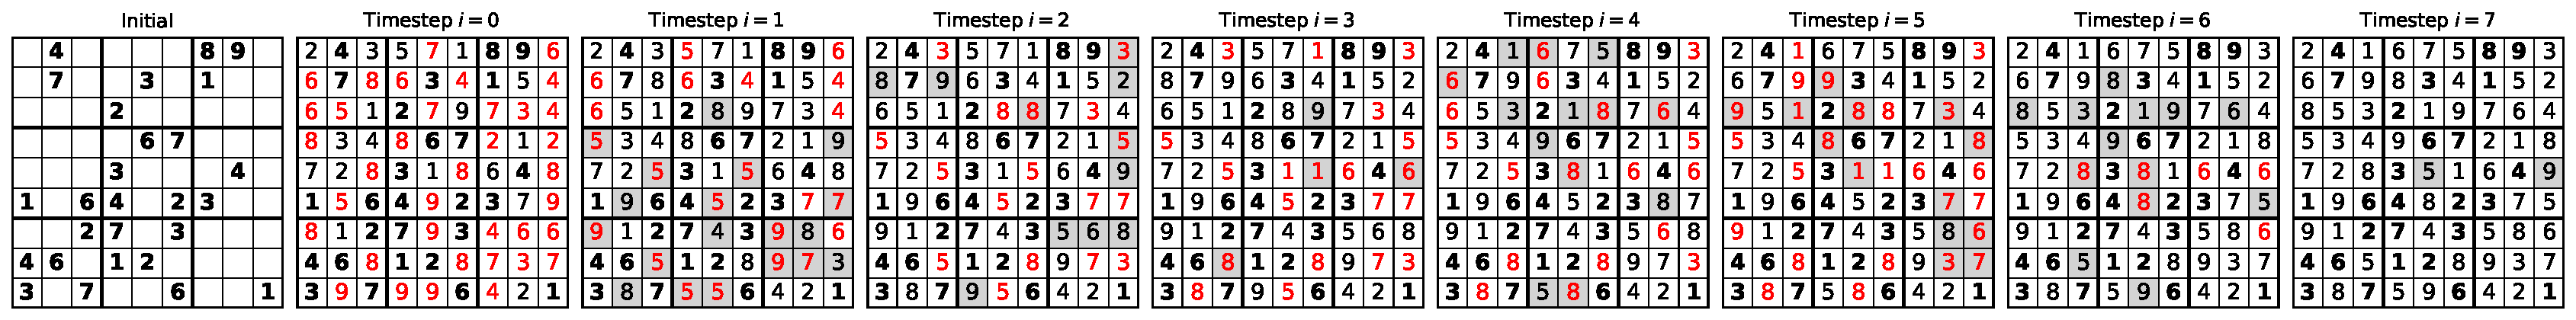
\includegraphics[width=1.1\linewidth]{figures/visualization/sudoku-hard-1.pdf}%
  }\\
    % row
  \makebox[\linewidth][c]{%
    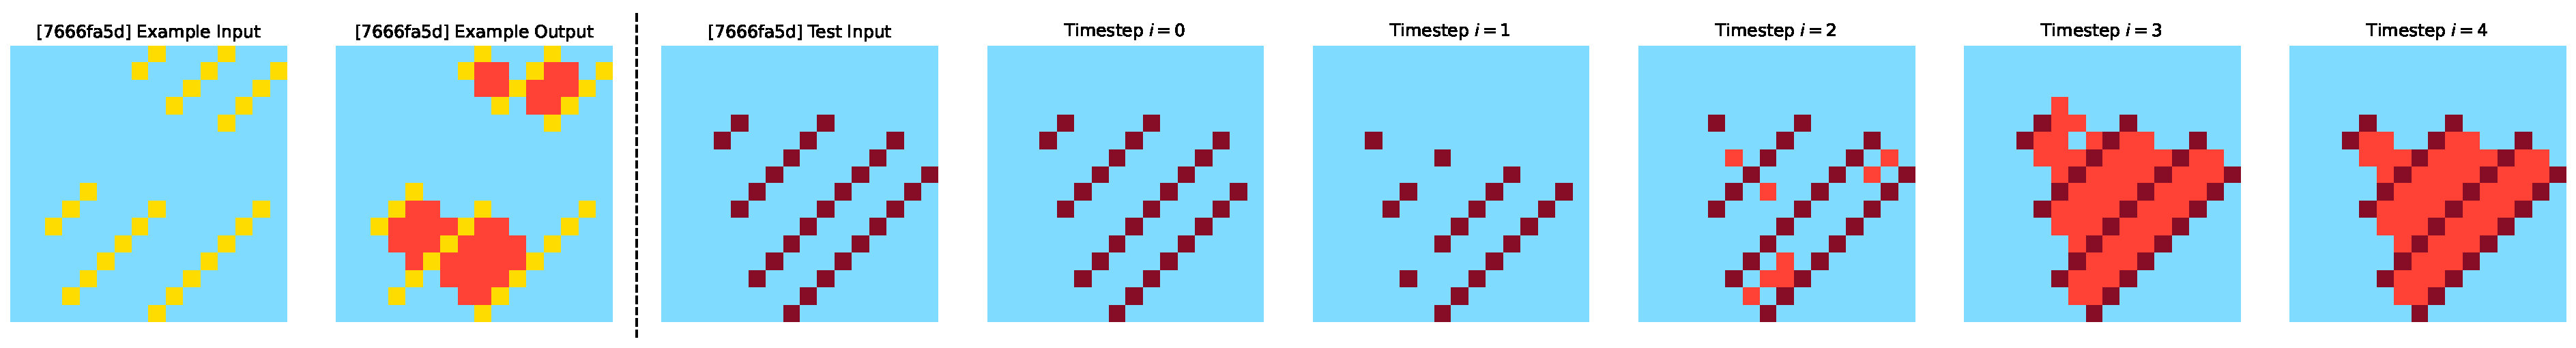
\includegraphics[width=1.1\linewidth]{figures/visualization/7666fa5d.pdf}%
  }\\
      % row
  \makebox[\linewidth][c]{%
    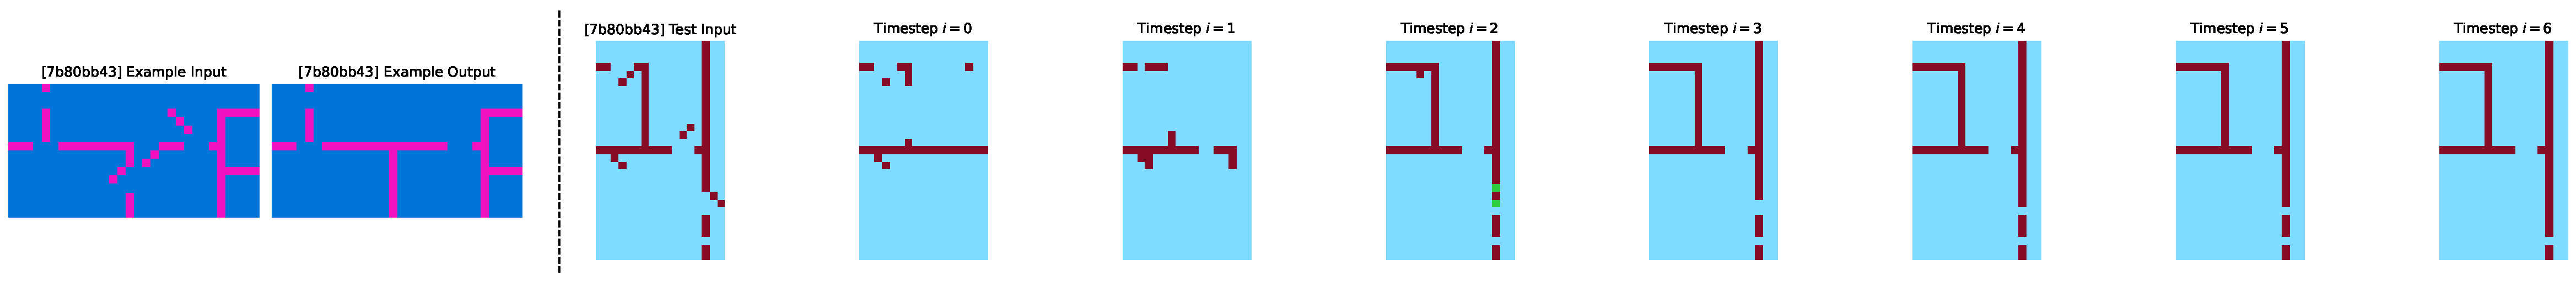
\includegraphics[width=1.1\linewidth]{figures/visualization/7b80bb43.pdf}%
  }
  \caption{\textbf{Visualization of intermediate predictions by HRM on benchmark tasks.} \textbf{Top:} \textit{Maze-Hard}—blue cells indicate the predicted path. \textbf{Middle:} \textit{Sudoku-Extreme}—bold cells represent initial givens; red highlights cells violating Sudoku constraints; grey shading indicates changes from the previous timestep.
  \textbf{Bottom:} ARC-AGI-2 Task—left: provided example input-output pair; right: intermediate steps solving the test input.}
  \label{fig:visualization}
\end{figure}

Inspired by this hierarchical and multi-timescale biological architecture, we propose the Hierarchical Reasoning Model (HRM). HRM is designed to significantly increase the effective computational depth. It features two coupled recurrent modules: a high-level (H) module for abstract, deliberate reasoning, and a low-level (L) module for fast, detailed computations. This structure avoids the rapid convergence of standard recurrent models through a process we term ``hierarchical convergence.'' The slow-updating H-module advances only after the fast-updating L-module has completed multiple computational steps and reached a local equilibrium, at which point the L-module is reset to begin a new computational phase.

Furthermore, we propose a one-step gradient approximation for training HRM, which offers improved efficiency and eliminates the requirement for BPTT. This design maintains a constant memory footprint ($O(1)$ compared to BPTT's $O(T)$ for $T$ timesteps) throughout the backpropagation process, making it scalable and more biologically plausible.

Leveraging its enhanced effective depth, HRM excels at tasks that demand extensive search and backtracking. \textbf{Using only 1,000 input-output examples, without pre-training or CoT supervision}, HRM learns to solve problems that are intractable for even the most advanced LLMs. For example, it achieves near-perfect accuracy in complex Sudoku puzzles (\textit{Sudoku-Extreme Full}) and optimal pathfinding in 30x30 mazes, where state-of-the-art CoT methods completely fail (0\% accuracy). In the Abstraction and Reasoning Corpus (ARC) AGI Challenge~\cite{AbstractionReasoning2019, Chollet2024ARCP2, Chollet2025ARCAGI2AN} - a benchmark of inductive reasoning - HRM, trained from scratch with only the official dataset (\textasciitilde1000 examples), with only 27M parameters and a 30x30 grid context (900 tokens), achieves a performance of \textbf{40.3\%}, which substantially surpasses leading CoT-based models like o3-mini-high (34.5\%) and Claude 3.7 8K context (21.2\%), despite their considerably larger parameter sizes and context lengths, as shown in \Cref{fig:benchmark_bars}. This represents a promising direction toward the development of next-generation AI reasoning systems with universal computational capabilities.
